
%\section[\textlatin{Codd Rules}]{\textgreek{Οι 12 κανόνες του} \textlatin{E.F. Codd}}

\section[\textlatin{Codd Rules}]{\textgreek{Οι 12 κανόνες του} \textlatin{Codd}}


\begin{frame}[t,fragile]
\frametitle{\en Edgar F. Codd}
\begin{columns}[T]
  \begin{column}{0.65\textwidth}
    \begin{itemize}
      \item Άγγλος επιστήμονας, 1923 -- 2003.
      \item Θεμελιωτής του σχεσιακού μοντέλου βάσεων δεδομένων.
      \item Πιλότος στο 2ο παγκόσμιο πόλεμο.
      \item Εργάστηκε πολλά χρόνια για την {\en IBM}.
      \item Περισσότερο γνωστός για την εργασία του 
           {\en\color{blue} "A Relational Model of Data for Large Shared Data Banks".\footnote{\url{http://dl.acm.org/citation.cfm?doid=362384.362685}}}
      \item Βραβείο {\sq Turing} το 1981.     
    \end{itemize}
  \end{column}
  \begin{column}{0.35\textwidth} \hspace*{-2cm}
    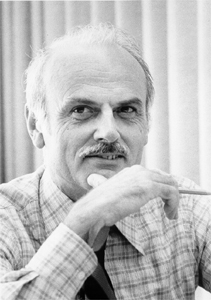
\includegraphics[scale=0.8]{Edgar_F_Codd.jpg}
  \end{column}
\end{columns}
\end{frame}



\begin{frame}[t,fragile]
\frametitle{Κανόνας $\# 1$ }
\begin{minipage}{\wE}
  \en
  \begin{bclogo} [couleur=colBC, logo=\bccrayon, arrondi=0.1, couleurBord=red!80!blue, barre=none] {The information Rule}
    \em
      All information in a relational database (including table and column names) is represented in only one way, namely as a value in a table.
  \end{bclogo}
  \el
  \begin{block}{\en The information rule}
     Όλα τα δεδομένα και οι πληροφορίες της βάσης αναπαριστώνται
     στο λογικό επίπεδο της βάσης δεδομένων μέσα σε πίνακες.
  \end{block}
\end{minipage}
\end{frame}



\begin{frame}[t,fragile]
\frametitle{Κανόνας $\# 2$ }
\begin{minipage}{\wE}
  \en
  \begin{bclogo} [couleur=colBC, logo=\bccrayon, arrondi=0.1, couleurBord=red!80!blue, barre=none] {The guaranteed access rule}
    \em
      All data must be accessible. 
      This rule is essentially a restatement of the fundamental requirement for primary keys. 
      It says that every individual scalar value in the database must be logically addressable 
      by specifying the name of the containing table, the name of the containing column 
      and the primary key value of the containing row.
  \end{bclogo}
  \el
  \begin{block}{\en The guaranteed access rule}
     Με βάση το λογικό επίπεδο της βάσης, όλα τα δεδομένα μπορούν
     να προσπελαστούν με βάση τον πίνακα στον οποίο έχουν καταχωρηθεί,
     με την τιμή του πρωτεύοντος κλειδιού, και το όνομα της στήλης του πίνακα.
  \end{block}
\end{minipage}
\end{frame}


\begin{frame}[t,fragile]
\frametitle{Κανόνας $\# 3$ }
\begin{minipage}{\wE}
  \en
  \begin{bclogo} [couleur=colBC, logo=\bccrayon, arrondi=0.1, couleurBord=red!80!blue, barre=none] {Systematic treatment of null values:}
    \em
      The DBMS must allow each field to remain null (or empty). Specifically, it must support a representation of "missing information and inapplicable information" that is systematic, distinct from all regular values (for example, "distinct from zero or any other number", in the case of numeric values), and independent of data type. 
      It is also implied that such representations must be manipulated by the DBMS in a systematic way.
  \end{bclogo}
  \el
  \begin{block}{}%{\en The guaranteed access rule}
     Οι τιμές {\sq \tnull} πρέπει να χρησιμοποιούνται ως ελλιπής πληροφορία,
        όχι ως μηδενικές αριθμητικές τιμές, κενά αλφαριθμητικά ή ο κενός
        χαρακτήρας (\men{space}).
  \end{block}
\end{minipage}
\end{frame}

